%% no need for  \DeclareGraphicsExtensions{.pdf,.eps}

\documentclass[12pt,letterpaper,english]{article}
\usepackage{times}
\usepackage[T1]{fontenc}
\IfFileExists{url.sty}{\usepackage{url}}
                      {\newcommand{\url}{\texttt}}

\usepackage{babel}
%\usepackage{noweb}
\usepackage{Rd}

\usepackage{Sweave}

%\VignetteIndexEntry{Performance Attribution from Bacon}
%\VignetteDepends{PerformanceAnalytics}
%\VignetteKeywords{returns, performance, risk, benchmark, portfolio}
%\VignettePackage{PerformanceAnalytics}

%\documentclass[a4paper]{article}
%\usepackage[noae]{Sweave}
%\usepackage{ucs}
%\usepackage[utf8x]{inputenc}
%\usepackage{amsmath, amsthm, latexsym}
%\usepackage[top=3cm, bottom=3cm, left=2.5cm]{geometry}
%\usepackage{graphicx}
%\usepackage{graphicx, verbatim}
%\usepackage{ucs}
%\usepackage[utf8x]{inputenc}
%\usepackage{amsmath, amsthm, latexsym}
%\usepackage{graphicx}

\title{Umsmooth Return Models Impact}
\author{Shubhankit Mohan}

\begin{document}
\Sconcordance{concordance:UnSmoothReturnAnalysis.tex:UnSmoothReturnAnalysis.Rnw:%
1 46 1 1 5 1 4 45 1 1 4 1 2 2 1 1 4 1 2 3 1 1 3 1 2 3 1 1 3 1 2 5 1 1 2 %
1 0 3 1 5 0 1 1 5 0 1 2 6 0 1 1 5 0 1 2 1 0 1 1 1 2 1 0 1 2 1 0 1 2 5 0 %
1 2 1 1 1 2 1 0 4 1 1 2 1 0 1 2 1 0 1 2 6 0 1 3 10 1 1 5 5 0 1 2 9 1 1 %
2 10 0 1 1 10 0 1 2 10 1 1 2 1 0 1 1 12 0 1 1 13 0 1 2 10 1 1 2 1 0 1 1 %
12 0 1 1 13 0 1 2 4 1 1 2 1 0 1 1 12 0 1 1 13 0 1 2 11 1 1 2 1 0 1 1 16 %
0 1 1 17 0 1 2 9 1 1 5 17 0 1 2 9 1 1 3 12 0 1 1 12 0 1 2 8 1 1 5 15 0 %
1 2 10 1 1 2 1 0 1 1 14 0 1 1 15 0 1 2 8 1 1 2 1 0 1 1 16 0 1 1 17 0 1 %
2 12 1 1 2 1 0 1 1 12 0 1 1 13 0 1 2 4 1 1 2 1 0 1 1 12 0 1 1 13 0 1 2 %
4 1 1 2 1 0 1 1 16 0 1 1 17 0 1 2 8 1 1 2 1 0 1 1 16 0 1 1 17 0 1 2 8 1 %
1 2 1 0 1 1 16 0 1 1 17 0 1 2 8 1 1 2 1 0 1 1 14 0 1 1 15 0 1 2 8 1 1 2 %
1 0 1 1 14 0 1 1 15 0 1 2 9 1 2 2 2 1 2 2 4 1 1 2 5 0 1 2 3 1 1 2 5 0 1 %
2 1 1}


\maketitle


\begin{abstract}
The fact that many hedge fund returns exhibit extraordinary levels of serial correlation is now well-known and generally accepted as fact.Because hedge fund strategies have exceptionally high autocorrelations in reported returns and this is taken as evidence of return smoothing, we first develop a method to completely eliminate any order of serial correlation across a wide array of time series processes.Once this is complete, we can determine the underlying risk factors to the "true" hedge fund returns and examine the incremental benefit attained from using nonlinear payoffs relative to the more traditional linear factors.
\end{abstract}
\tableofcontents




\section{Okunev White Model Methodology}
Given a sample of historical returns \((R_1,R_2, . . .,R_T)\),the method assumes the fund manager smooths returns in the following manner:

%Let $X \sim N(0,1)$ and $Y \sim \textrm{Exponential}(\mu)$.  Let
%$Z = \sin(X)$. $\sqrt{X}$.
  
%$\hat{\mu}$ = $\displaystyle\frac{22}{7}$
%e^{2 \mu} = 1
%\begin{equation}
%\left(\sum_{t=1}^{T} R_t/T\right) = \hat{\mu} \\
%\end{equation}
\begin{equation}
 r_{0,t}  =  \sum_{i}^{} \beta_{i}r_{0,t-i} + (1- \alpha)r_{m,t} \\
\end{equation}


\begin{equation}
where :  \sum_{i}^{} \beta_{i} = (1- \alpha) \\
\end{equation}

\(r_{0,t}\) : is the observed (reported) return at time t (with 0 adjustments' to reported returns), \\
\(r_{m,t}\) : is the true underlying (unreported) return at time t (determined by making m adjustments to reported returns). \\

The objective is to determine the true underlying return by removing the
autocorrelation structure in the original return series without making any assumptions regarding the actual time series properties of the underlying process. We are implicitly assuming by this approach that the autocorrelations that arise in reported returns are entirely due to the smoothing behavior funds engage in when reporting results. In fact, the method may be adopted to produce any desired level of autocorrelation at any lag and is not limited to simply eliminating all autocorrelations.

\section{To Remove Up to m Orders of Autocorrelation}
To remove the first m orders of autocorrelation from a given return series we would proceed in a manner very similar to that detailed in \textbf{Geltner Return}. We would initially remove the first order autocorrelation, then proceed to eliminate the second order autocorrelation through the iteration process. In general, to remove any order, m, autocorrelations from a given return series we would make the following transformation to returns:

\begin{equation}
r_{m,t}=\frac{r_{m-1,t}-c_{m}r_{m-1,t-m}}{1-c_{m}}
\end{equation}

Where  \(r_{m-1,t}\) is the series return with the first (m-1) order autocorrelation coefficient's removed.The general form for all the autocorrelations given by the process is : 
\begin{equation}
a_{m,n}=\frac{a_{m-1,n}(1+c_{m}^2)-c_{m}(1+a_{m-1,2m})}{1+c_{m}^2 -2c_{m}a_{m-1,n}}
\end{equation}

Once a solution is found for \(c_{m}\) to create \(r_{m,t}\) , one will need to iterate back to remove the first 'm'autocorrelations again. One will then need to once again remove the mth autocorrelation using the adjustment in equation (3). It would continue the process until the first m autocorrelations are sufficiently close to zero.

\section{Time Series Characteristics}

Given a series  of historical returns \((R_1,R_2, . . .,R_T)\) from \textbf{January-1997} to \textbf{January-2008}, create a wealth index chart, bars for per-period performance, and underwater chart for drawdown of the  Hedge Funds Indiciesfrom EDHEC Database.

\subsection{ Performance Summary}
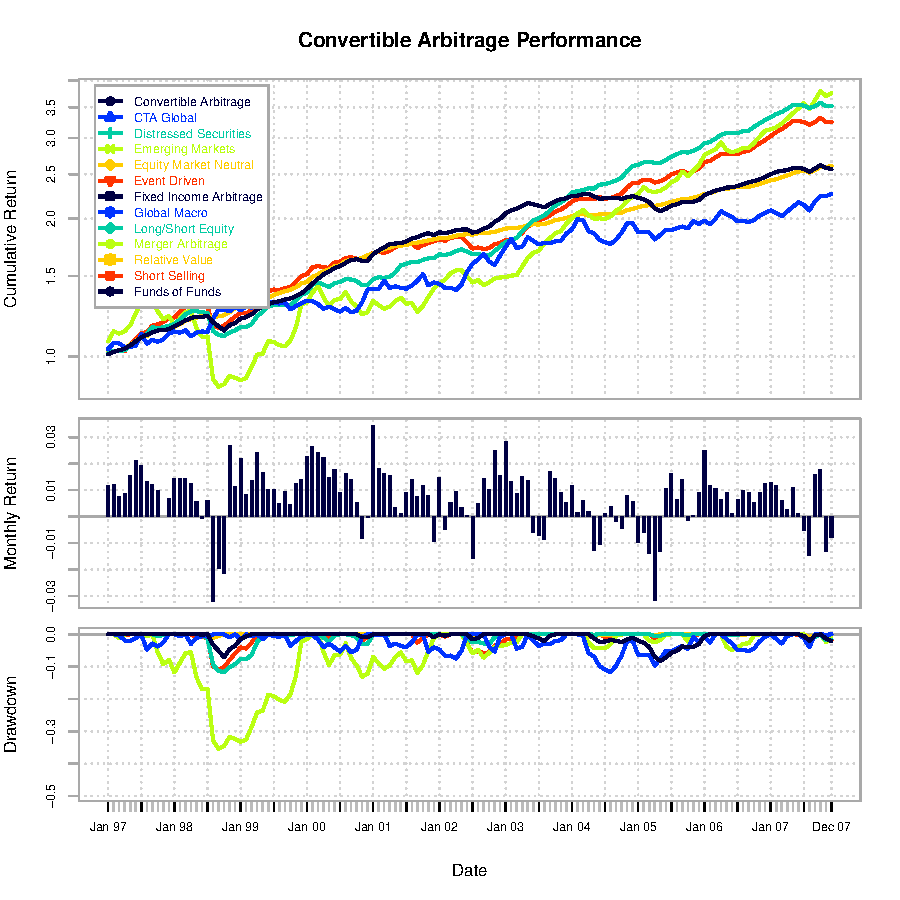
\includegraphics{UnSmoothReturnAnalysis-003}

After applying the \textbf{Okunev White Model} to remove the serial correlation , we get the following Performance Chart.

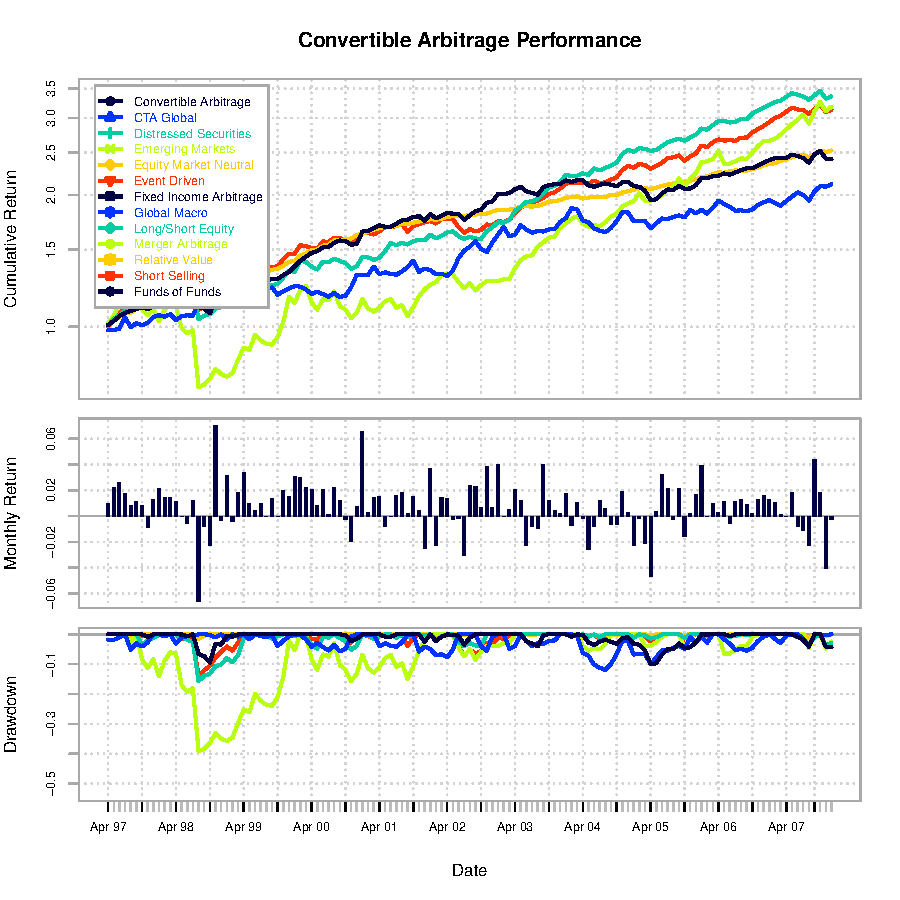
\includegraphics{UnSmoothReturnAnalysis-004}

\subsection{Autocorrelation UnSmoothing Impact}
One promiment feature visible by the summary chart is the removal of \textbf{serial autocorrelation} and \textbf{unsoomthing} of the return series.The significant drop in autocorrelation, is visible by the following chart based on  indicies of the CTA global ,Distressed Securities and Ememrging Markets which had the highest autocorrelation .

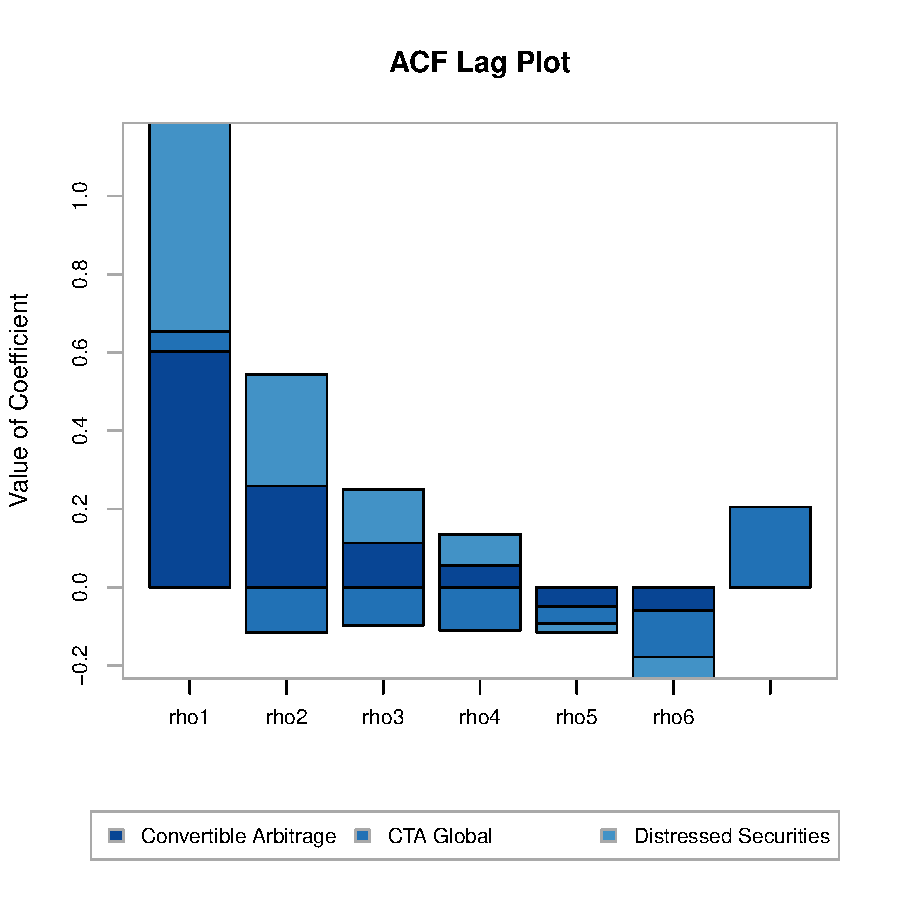
\includegraphics{UnSmoothReturnAnalysis-005}

The change can be evidently seen by the following chart :


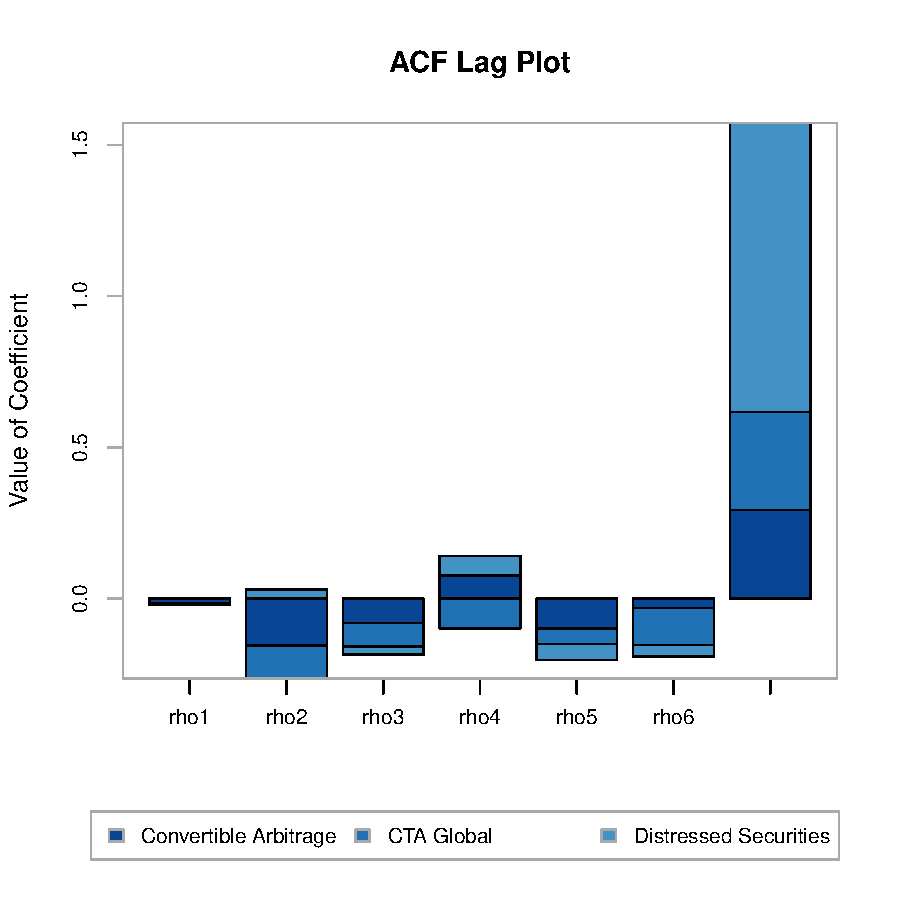
\includegraphics{UnSmoothReturnAnalysis-006}


\subsection{Comparing Distributions}

In this example we use edhec database, to compute true Hedge Fund Returns.

\begin{Schunk}
\begin{Sinput}
> library(PerformanceAnalytics)
> data(edhec)
> Returns = Return.Okunev(edhec[,1])
> skewness(edhec[,1])
\end{Sinput}
\begin{Soutput}
[1] -2.683657
\end{Soutput}
\begin{Sinput}
> skewness(Returns)
\end{Sinput}
\begin{Soutput}
[1] -1.19068
\end{Soutput}
\begin{Sinput}
> # Right Shift of Returns Ditribution for a negative skewed distribution 
> kurtosis(edhec[,1])
\end{Sinput}
\begin{Soutput}
[1] 16.17819
\end{Soutput}
\begin{Sinput}
> kurtosis(Returns)
\end{Sinput}
\begin{Soutput}
[1] 10.59337
\end{Soutput}
\begin{Sinput}
> # Reduction in "peakedness" around the mean
> layout(rbind(c(1, 2), c(3, 4)))
>  chart.Histogram(Returns, main = "Plain", methods = NULL)
>  chart.Histogram(Returns, main = "Density", breaks = 40,
+  methods = c("add.density", "add.normal"))
>  chart.Histogram(Returns, main = "Skew and Kurt",
+  methods = c("add.centered", "add.rug"))
> chart.Histogram(Returns, main = "Risk Measures",
+  methods = c("add.risk"))
\end{Sinput}
\end{Schunk}
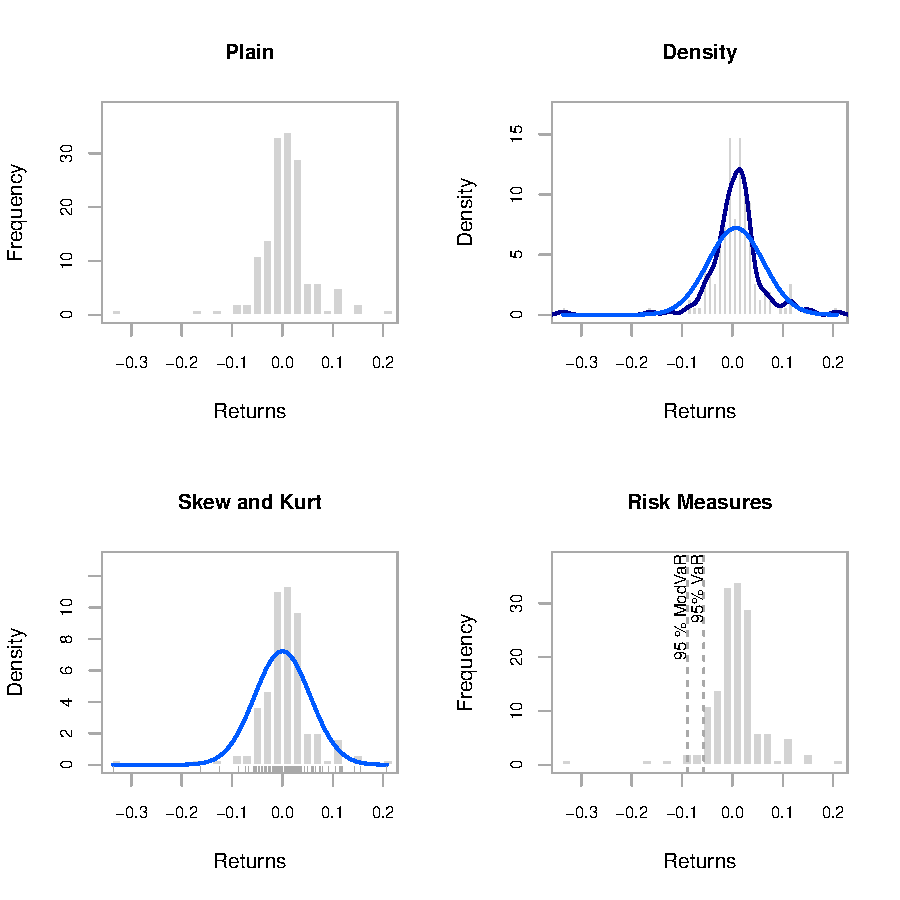
\includegraphics{UnSmoothReturnAnalysis-007}

The above figure shows the behaviour of the distribution tending to a normal IID distribution.For comparitive purpose, one can observe the change in the charateristics of return as compared to the orignal.
\begin{Schunk}
\begin{Sinput}
> library(PerformanceAnalytics)
> data(edhec)
> Returns = Return.Okunev(edhec[,1])
> layout(rbind(c(1, 2), c(3, 4)))
>  chart.Histogram(edhec[,1], main = "Plain", methods = NULL)
>  chart.Histogram(edhec[,1], main = "Density", breaks = 40,
+  methods = c("add.density", "add.normal"))
>  chart.Histogram(edhec[,1], main = "Skew and Kurt",
+  methods = c("add.centered", "add.rug"))
> chart.Histogram(edhec[,1], main = "Risk Measures",
+  methods = c("add.risk"))
> 
\end{Sinput}
\end{Schunk}
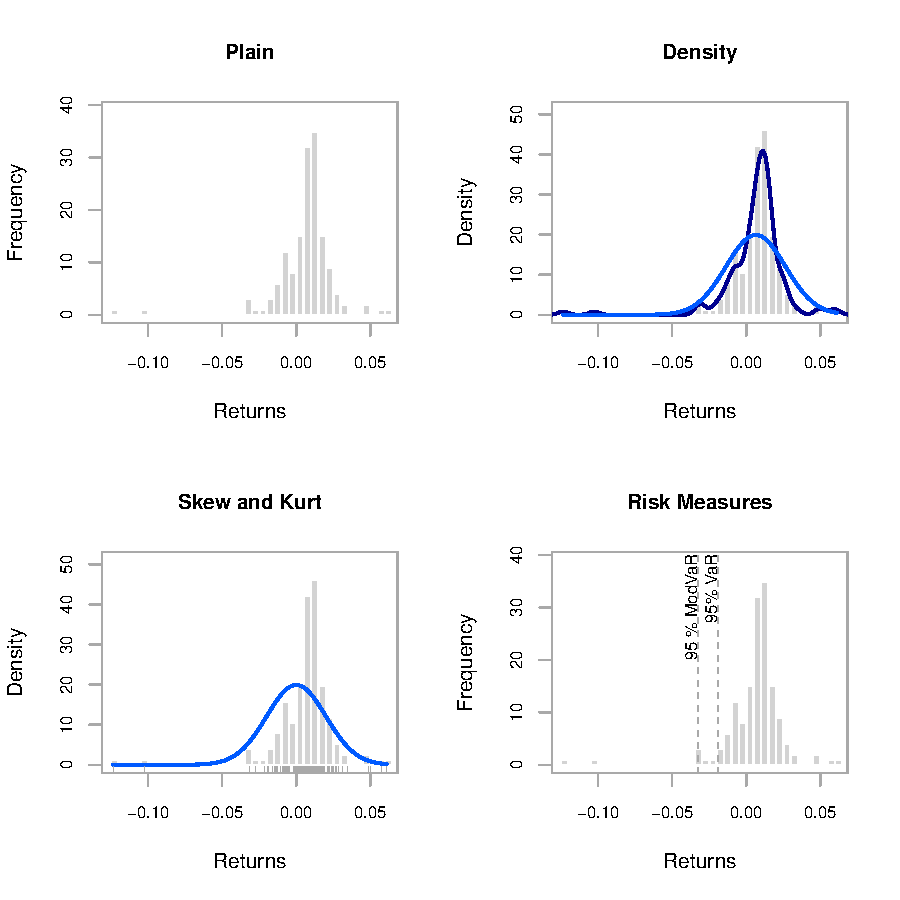
\includegraphics{UnSmoothReturnAnalysis-008}

\section{Risk Measure}

\subsection{Mean absolute deviation}

To calculate Mean absolute deviation we take the sum of the absolute value of the difference between the returns and the mean of the returns and we divide it by the number of returns.

 \deqn{MeanAbsoluteDeviation = \frac{\sum^{n}_{i=1}\mid r_i - \overline{r}\mid}{n}}{MeanAbsoluteDeviation = sum(|r-mean(r)|)/n }

where \eqn{n} is the number of observations of the entire series, \eqn{r_i} is the return in month i and \eqn{\overline{r}} is the mean return

\begin{Schunk}
\begin{Soutput}
                        Convertible Arbitrage CTA Global Distressed Securities
Mean absolute deviation              191.5453   5.581807              89.59503
\end{Soutput}
\end{Schunk}

We can observe than due to the spurious serial autocorrelation, the true \textbf{volatility} was hidden, which is \textbf{more than 100 \% } in case of Distressed Securities to the one apparent to the investor.\textbf{CTA Global}, has the lowerst change, which is consistent,with the fact with it has the lowest autocorreration.


\subsection{Sharpe Ratio}

The Sharpe ratio is simply the return per unit of risk (represented by variability).  In the classic case, the unit of risk is the standard deviation of the returns.
 
\deqn{\frac{\overline{(R_{a}-R_{f})}}{\sqrt{\sigma_{(R_{a}-R_{f})}}}}

\begin{Schunk}
\begin{Soutput}
                              Convertible Arbitrage CTA Global
StdDev Sharpe (Rf=0%, p=95%):            0.31967021  0.2582269
VaR Sharpe (Rf=0%, p=95%):               0.19734443  0.1919833
ES Sharpe (Rf=0%, p=95%):                0.06437672  0.1514751
                              Distressed Securities
StdDev Sharpe (Rf=0%, p=95%):             0.4334711
VaR Sharpe (Rf=0%, p=95%):                0.2892904
ES Sharpe (Rf=0%, p=95%):                 0.1306556
\end{Soutput}
\begin{Soutput}
                              Convertible Arbitrage CTA Global
StdDev Sharpe (Rf=0%, p=95%):            0.12060647  0.2330569
VaR Sharpe (Rf=0%, p=95%):               0.07461253  0.1689703
ES Sharpe (Rf=0%, p=95%):                0.02832469  0.1328497
                              Distressed Securities
StdDev Sharpe (Rf=0%, p=95%):            0.24494271
VaR Sharpe (Rf=0%, p=95%):               0.14988705
ES Sharpe (Rf=0%, p=95%):                0.07186104
\end{Soutput}
\end{Schunk}

The Sharpe Ratio should expectedly fall, as in UnSmooth Return model, the returns decrease and standard deveation increases simaltaneously.\textbf{CTA Global}, is the sole index, which does not experience a sharp fall, which can be attributed to the low autocorrelation coefficient \textbf{(0.05)}. 

\subsection{Value at Risk }

Value at Risk (VaR) has become a required standard risk measure recognized by Basel II and MiFID.Traditional mean-VaR may be derived historically, or estimated parametrically using
        \deqn{                z_{c} = q_{p}=qnorm(p)}

\deqn{               VaR=\bar{R} -  z_{c} \cdot \sqrt{\sigma}}


\begin{Schunk}
\begin{Sinput}
> data(edhec)
> VaR(edhec, p=.95, method="gaussian")
\end{Sinput}
\begin{Soutput}
    Convertible Arbitrage  CTA Global Distressed Securities Emerging Markets
VaR           -0.02645782 -0.03471098            -0.0221269      -0.05498927
    Equity Market Neutral Event Driven Fixed Income Arbitrage Global Macro
VaR          -0.008761813  -0.02246202            -0.01900198  -0.02023018
    Long/Short Equity Merger Arbitrage Relative Value Short Selling
VaR       -0.02859264      -0.01152478    -0.01493049   -0.08617027
    Funds of Funds
VaR    -0.02393888
\end{Soutput}
\begin{Sinput}
> VaR(Return.Okunev(edhec), p=.95, method="gaussian") 
\end{Sinput}
\begin{Soutput}
    Convertible Arbitrage  CTA Global Distressed Securities Emerging Markets
VaR           -0.08394453 -0.03724858           -0.04617951      -0.07864815
    Equity Market Neutral Event Driven Fixed Income Arbitrage Global Macro
VaR           -0.01238121   -0.0372441            -0.04178068  -0.02143809
    Long/Short Equity Merger Arbitrage Relative Value Short Selling
VaR       -0.03983483      -0.01841034    -0.02907754    -0.1026801
    Funds of Funds
VaR    -0.03504775
\end{Soutput}
\end{Schunk}

\section{Regression analysis}

\subsection{Regression equation}

\deqn{r_P = \alpha + \beta * b + \epsilon}

\subsection{Regression alpha }

"Alpha" purports to be a measure of a manager's skill by measuring the portion of the managers returns that are not attributable to "Beta", or the portion of performance attributable to a benchmark.

\begin{Schunk}
\begin{Sinput}
> data(managers)
> CAPM.alpha(edhec, managers[,8,drop=FALSE], Rf=.035/12)
\end{Sinput}
\begin{Soutput}
                Convertible Arbitrage  CTA Global Distressed Securities
Alpha: SP500 TR           0.004471465 0.003821383            0.00636263
                Emerging Markets Equity Market Neutral Event Driven
Alpha: SP500 TR      0.004841242           0.004170222  0.005182049
                Fixed Income Arbitrage Global Macro Long/Short Equity
Alpha: SP500 TR            0.002324711  0.004706408       0.005009663
                Merger Arbitrage Relative Value Short Selling Funds of Funds
Alpha: SP500 TR      0.003935414    0.004268617   0.005397325    0.003917601
\end{Soutput}
\begin{Sinput}
> CAPM.alpha(Return.Okunev(edhec), managers[,8,drop=FALSE], Rf=.035/12)
\end{Sinput}
\begin{Soutput}
                Convertible Arbitrage  CTA Global Distressed Securities
Alpha: SP500 TR           0.003623436 0.003482153           0.005457597
                Emerging Markets Equity Market Neutral Event Driven
Alpha: SP500 TR      0.003004784           0.004048946  0.004523336
                Fixed Income Arbitrage Global Macro Long/Short Equity
Alpha: SP500 TR             0.00184902  0.004405292       0.004630361
                Merger Arbitrage Relative Value Short Selling Funds of Funds
Alpha: SP500 TR       0.00365762    0.003672505   0.005288907    0.003442342
\end{Soutput}
\end{Schunk}

\subsection{Regression beta}

CAPM Beta is the beta of an asset to the variance and covariance of an initial portfolio.  Used to determine diversification potential.

\begin{Schunk}
\begin{Sinput}
> data(managers)
> CAPM.beta(edhec, managers[, "SP500 TR", drop=FALSE], Rf = managers[, "US 3m TR", drop=FALSE])
\end{Sinput}
\begin{Soutput}
               Convertible Arbitrage  CTA Global Distressed Securities
Beta: SP500 TR            0.04824155 -0.07328212             0.1692722
               Emerging Markets Equity Market Neutral Event Driven
Beta: SP500 TR        0.5092851            0.05648291    0.2379033
               Fixed Income Arbitrage Global Macro Long/Short Equity
Beta: SP500 TR           -0.009447579    0.1664831         0.3368761
               Merger Arbitrage Relative Value Short Selling Funds of Funds
Beta: SP500 TR        0.1357786      0.1356442     -1.000142      0.2145575
\end{Soutput}
\begin{Sinput}
> CAPM.beta(Return.Okunev(edhec), managers[, "SP500 TR", drop=FALSE], Rf = managers[, "US 3m TR", drop=FALSE])
\end{Sinput}
\begin{Soutput}
               Convertible Arbitrage  CTA Global Distressed Securities
Beta: SP500 TR             0.2324435 -0.08548672             0.3996316
               Emerging Markets Equity Market Neutral Event Driven
Beta: SP500 TR        0.7753848            0.07331462    0.4013961
               Fixed Income Arbitrage Global Macro Long/Short Equity
Beta: SP500 TR             0.03619617    0.1681044         0.4535646
               Merger Arbitrage Relative Value Short Selling Funds of Funds
Beta: SP500 TR         0.199134      0.2684195     -1.177247       0.318659
\end{Soutput}
\end{Schunk}

This is an \textbf{interesting} find of investigation.\textbf{Contorary}, to the belief , that \emph{umsmoothing the returns would make it more volatile, with idiosyncratic components}, the regression shows, that the true returns are \textbf{much more} significantly related to Financial Markets, as compared to the visible returns to the investors.This also weakens the belief, that hedge funds give returns, irrespective of the market conditions. 


\subsection{Jensen's alpha }

The Jensen's alpha is the intercept of the regression equation in the Capital Asset Pricing Model and is in effect the exess return adjusted for systematic risk.

\deqn{\alpha = r_p - r_f - \beta_p * (b - r_f)}{alpha = r_p - r_f - beta_p * (b - r_f)}

where \eqn{r_f}. is the risk free rate, \eqn{\beta_r}. is the regression beta, \eqn{r_p}. is the portfolio return and b is the benchmark return

\begin{Schunk}
\begin{Sinput}
> data(edhec)
> CAPM.jensenAlpha(edhec,managers[,8],Rf=.03/12)
\end{Sinput}
\begin{Soutput}
                                    Convertible Arbitrage CTA Global
Jensen's Alpha (Risk free = 0.0025)            0.06999936  0.0812573
                                    Distressed Securities Emerging Markets
Jensen's Alpha (Risk free = 0.0025)            0.07949484       0.04377234
                                    Equity Market Neutral Event Driven
Jensen's Alpha (Risk free = 0.0025)            0.06617577   0.06851869
                                    Fixed Income Arbitrage Global Macro
Jensen's Alpha (Risk free = 0.0025)              0.0493231   0.07618595
                                    Long/Short Equity Merger Arbitrage
Jensen's Alpha (Risk free = 0.0025)        0.05988859       0.06845796
                                    Relative Value Short Selling Funds of Funds
Jensen's Alpha (Risk free = 0.0025)     0.06714829     0.1240347     0.04870534
\end{Soutput}
\begin{Sinput}
> CAPM.jensenAlpha(Return.Okunev(edhec),managers[,8],Rf=.03/12)
\end{Sinput}
\begin{Soutput}
                                    Convertible Arbitrage CTA Global
Jensen's Alpha (Risk free = 0.0025)            0.03808553 0.07805832
                                    Distressed Securities Emerging Markets
Jensen's Alpha (Risk free = 0.0025)            0.05490376      0.002827883
                                    Equity Market Neutral Event Driven
Jensen's Alpha (Risk free = 0.0025)            0.06349135   0.05133152
                                    Fixed Income Arbitrage Global Macro
Jensen's Alpha (Risk free = 0.0025)             0.03995779    0.0726611
                                    Long/Short Equity Merger Arbitrage
Jensen's Alpha (Risk free = 0.0025)        0.04786047       0.06170853
                                    Relative Value Short Selling Funds of Funds
Jensen's Alpha (Risk free = 0.0025)     0.05300399     0.1250439     0.03648212
\end{Soutput}
\end{Schunk}

The Jensen's alpha diminish significantly with Okunev Return model.However, with \textbf{CTA Global}, the alpha does not change by more than 3\% .
\subsection{Systematic Risk}

Systematic risk as defined by Bacon(2008) is the product of beta by market risk. Be careful ! It's not the same definition as the one given by Michael Jensen. Market risk is the standard deviation of the benchmark. The systematic risk is annualized

\deqn{\sigma_s = \beta * \sigma_m}{systematic risk = beta * market risk}

where \eqn{\sigma_s}. is the systematic risk, \eqn{\beta}. is the regression beta, and \eqn{\sigma_m} is the market risk

\begin{Schunk}
\begin{Soutput}
                                     Convertible Arbitrage CTA Global
Systematic Risk to SP500 TR (Rf = 0)              382.1817   18.46926
                                     Distressed Securities Emerging Markets
Systematic Risk to SP500 TR (Rf = 0)              139.0751         52.54349
                                     Equity Market Neutral Event Driven
Systematic Risk to SP500 TR (Rf = 0)              27.61317     68.90475
                                     Fixed Income Arbitrage Global Macro
Systematic Risk to SP500 TR (Rf = 0)               157.3361   0.02542014
                                     Long/Short Equity Merger Arbitrage
Systematic Risk to SP500 TR (Rf = 0)          34.37248         45.69652
                                     Relative Value Short Selling
Systematic Risk to SP500 TR (Rf = 0)       97.82683      17.98637
                                     Funds of Funds
Systematic Risk to SP500 TR (Rf = 0)       48.21903
\end{Soutput}
\end{Schunk}

The above table shows, the increase in \% of the market risk\eqn{\sigma_m}, after Okunev White model has been implemented.Concurrent with the investment stlye, \textbf{Equity Market Neutral, Short Selling , Global Macro} show least amount of indifference to their market risk exposure.


\subsection{Treynor ratio }

The Treynor ratio is similar to the Sharpe Ratio, except it uses beta as the volatility measure (to divide the investment's excess return over the beta).It is a performance metric that measures the effective return adjusted for market risk. Well-diversified portfolios should have similar Sharpe and Treynor Ratios because the standard deviation reduces to the beta.

\deqn{TreynorRatio = \frac{\overline{(R_{a}-R_{f})}}{\beta_{a,b}}}{(mean(Ra-Rf))/(Beta(Ra,Rb))}

\begin{Schunk}
\begin{Soutput}
                        Convertible Arbitrage CTA Global Distressed Securities
Treynor Ratio: SP500 TR                0.8368    -0.5328                0.3644
                        Emerging Markets Equity Market Neutral Event Driven
Treynor Ratio: SP500 TR           0.1119                0.6658       0.2372
                        Fixed Income Arbitrage Global Macro Long/Short Equity
Treynor Ratio: SP500 TR                -1.2009       0.3448            0.1687
                        Merger Arbitrage Relative Value Short Selling
Treynor Ratio: SP500 TR           0.3444         0.3368        0.0029
                        Funds of Funds
Treynor Ratio: SP500 TR         0.1624
\end{Soutput}
\begin{Soutput}
                        Convertible Arbitrage CTA Global Distressed Securities
Treynor Ratio: SP500 TR                 0.112    -0.4005                 0.145
                        Emerging Markets Equity Market Neutral Event Driven
Treynor Ratio: SP500 TR            0.053                 0.505       0.1358
                        Fixed Income Arbitrage Global Macro Long/Short Equity
Treynor Ratio: SP500 TR                 0.3037        0.324             0.123
                        Merger Arbitrage Relative Value Short Selling
Treynor Ratio: SP500 TR           0.2318         0.1639        0.0155
                        Funds of Funds
Treynor Ratio: SP500 TR         0.1017
\end{Soutput}
\end{Schunk}

\textbf{CTA Global} has a negative value, which imply  as risk-free rate is less than the expected return, but the beta is negative. This means that the fund manger has performed well, managing to reduce risk but getting a return better than the risk free rate

\subsection{Downside Risk}
As we have obtained the true hedge fund returns, what is the actual \textbf{VaR,drawdown and downside potential} of the indices, can be illustrated by the following example, where we CTA Global and Distressed Securities indicies have been taken as sample data sets.

The following table, shows the change in \textbf{absolute value} in terms of percentage, when the Okunev White Return model has been implemented as compared to the Orginal model. We can observe, that for the given period , before the 2008 financial crisis, the hedge fund returns have a \textbf{100} \% increase in exposure.The result is consistent , when tested on other indicies, which show that true risk was camouflaged under the haze of smoothing in the hedge fund industry.


\begin{Schunk}
\begin{Soutput}
                             CTA Global Distressed Securities
Semi Deviation                 5.780347              75.67568
Gain Deviation                 1.775148              70.19231
Loss Deviation                 7.407407              48.18653
Downside Deviation (MAR=10%)   6.521739              75.16779
Downside Deviation (Rf=0%)     8.759124              89.07563
Downside Deviation (0%)        8.759124              89.07563
Maximum Drawdown               2.568493              17.88831
Historical VaR (95%)           5.932203              86.24339
Historical ES (95%)            5.518764              77.75176
Modified VaR (95%)             7.988166              96.72727
Modified ES (95%)              8.644860              85.38588
\end{Soutput}
\end{Schunk}



\section{Relative Risk}

\subsection{Tracking error}

A measure of the unexplained portion of performance relative to a benchmark.Tracking error is calculated by taking the square root of the average of the squared deviations between the investment's returns and the benchmark's returns, then multiplying the result by the square root of the scale of the returns.

\deqn{ TrackingError = \sqrt{\sum\frac{(R_{a}-R_{b})^{2}}{len(R_{a})\sqrt{scale}}} }{ TrackingError = sqrt(sum(Ra - Rb)^2 / (length(R) - 1)) * sqrt(scale)}

\begin{Schunk}
\begin{Sinput}
> data(managers)
> TrackingError(edhec, managers[,8,drop=FALSE]) 
\end{Sinput}
\begin{Soutput}
                         Convertible Arbitrage CTA Global Distressed Securities
Tracking Error: SP500 TR             0.1543707  0.1685952             0.1539006
                         Emerging Markets Equity Market Neutral Event Driven
Tracking Error: SP500 TR        0.1950528             0.1423184    0.1517637
                         Fixed Income Arbitrage Global Macro Long/Short Equity
Tracking Error: SP500 TR              0.1458036    0.1529016          0.157304
                         Merger Arbitrage Relative Value Short Selling
Tracking Error: SP500 TR        0.1412594      0.1452275     0.2391201
                         Funds of Funds
Tracking Error: SP500 TR      0.1524484
\end{Soutput}
\begin{Sinput}
> TrackingError(Return.Okunev(edhec), managers[,8,drop=FALSE]) 
\end{Sinput}
\begin{Soutput}
                         Convertible Arbitrage CTA Global Distressed Securities
Tracking Error: SP500 TR             0.2445393  0.1725162              0.187338
                         Emerging Markets Equity Market Neutral Event Driven
Tracking Error: SP500 TR        0.2375463             0.1474357     0.176381
                         Fixed Income Arbitrage Global Macro Long/Short Equity
Tracking Error: SP500 TR               0.183249    0.1623801         0.1801033
                         Merger Arbitrage Relative Value Short Selling
Tracking Error: SP500 TR        0.1551378      0.1655992      0.246828
                         Funds of Funds
Tracking Error: SP500 TR      0.1730591
\end{Soutput}
\end{Schunk}

\subsection{Information ratio }

The Active Premium divided by the Tracking Error.
 
InformationRatio = ActivePremium/TrackingError
 
This relates the degree to which an investment has beaten the benchmark to the consistency with which the investment has beaten the benchmark.

\begin{Schunk}
\begin{Sinput}
> data(managers)
> InformationRatio(edhec, managers[,8,drop=FALSE]) 
\end{Sinput}
\begin{Soutput}
                            Convertible Arbitrage  CTA Global
Information Ratio: SP500 TR            0.06641876 -0.05510777
                            Distressed Securities Emerging Markets
Information Ratio: SP500 TR             0.2728265        0.1837459
                            Equity Market Neutral Event Driven
Information Ratio: SP500 TR            0.05213518    0.2018958
                            Fixed Income Arbitrage Global Macro
Information Ratio: SP500 TR             -0.1439689    0.1284569
                            Long/Short Equity Merger Arbitrage Relative Value
Information Ratio: SP500 TR         0.2147325       0.06278675     0.09164164
                            Short Selling Funds of Funds
Information Ratio: SP500 TR    -0.2589545     0.08212568
\end{Soutput}
\begin{Sinput}
> abs(InformationRatio(Return.Okunev(edhec), managers[,8,drop=FALSE])) 
\end{Sinput}
\begin{Soutput}
                            Convertible Arbitrage CTA Global
Information Ratio: SP500 TR            0.01739878 0.08246386
                            Distressed Securities Emerging Markets
Information Ratio: SP500 TR             0.2154123       0.08186685
                            Equity Market Neutral Event Driven
Information Ratio: SP500 TR            0.04971605    0.1709152
                            Fixed Income Arbitrage Global Macro
Information Ratio: SP500 TR              0.1428086   0.09947874
                            Long/Short Equity Merger Arbitrage Relative Value
Information Ratio: SP500 TR         0.1907038       0.05806339     0.07847608
                            Short Selling Funds of Funds
Information Ratio: SP500 TR     0.3250201     0.06674165
\end{Soutput}
\end{Schunk}

\textbf{Short Selling} has the highest value as the returns produced by this fund have low correlation with the market returns.

\section{Drawdown}

\subsection{Pain index}

The pain index is the mean value of the drawdowns over the entire analysis period. The measure is similar to the Ulcer index except that the drawdowns are not squared.  Also, it's different than the average drawdown, in that the numerator is the total number of observations rather than the number of drawdowns. Visually, the pain index is the area of the region that is enclosed by the horizontal line at zero percent and the drawdown line in the Drawdown chart.

\deqn{Pain index = \sum^{n}_{i=1} \frac{\mid D'_i \mid}{n}}{Pain index = sum(|D'i|/n)}

where \eqn{n}. is the number of observations of the entire series, \eqn{D'_i}. is the drawdown since previous peak in period i

\begin{Schunk}
\begin{Sinput}
> data(edhec)
> print(PainIndex(edhec[,]))
\end{Sinput}
\begin{Soutput}
           Convertible Arbitrage CTA Global Distressed Securities
Pain Index            0.02515669 0.02330895            0.02427166
           Emerging Markets Equity Market Neutral Event Driven
Pain Index       0.08077422           0.008118339   0.02245003
           Fixed Income Arbitrage Global Macro Long/Short Equity
Pain Index             0.01783657   0.01035735        0.03111831
           Merger Arbitrage Relative Value Short Selling Funds of Funds
Pain Index      0.006876259     0.01253914     0.2192711     0.02395462
\end{Soutput}
\begin{Sinput}
> print(PainIndex(Return.Okunev(edhec[,])))
\end{Sinput}
\begin{Soutput}
           Convertible Arbitrage CTA Global Distressed Securities
Pain Index            0.04347953 0.02519844            0.03675718
           Emerging Markets Equity Market Neutral Event Driven
Pain Index        0.0933349           0.009222145   0.02850331
           Fixed Income Arbitrage Global Macro Long/Short Equity
Pain Index             0.02460773   0.01109697        0.03728646
           Merger Arbitrage Relative Value Short Selling Funds of Funds
Pain Index      0.009386586     0.01790537     0.2460317     0.03089789
\end{Soutput}
\end{Schunk}

\subsection{Calmar ratio}

Calmar ratio is another method of creating a risk-adjusted measure for ranking investments similar to the Sharpe ratio.

\begin{Schunk}
\begin{Sinput}
> data(managers)
> CalmarRatio(edhec)
\end{Sinput}
\begin{Soutput}
             Convertible Arbitrage CTA Global Distressed Securities
Calmar Ratio              0.263148  0.6569514             0.4253743
             Emerging Markets Equity Market Neutral Event Driven
Calmar Ratio        0.2601868             0.6671512    0.4640555
             Fixed Income Arbitrage Global Macro Long/Short Equity
Calmar Ratio              0.2834293     1.189059         0.4308705
             Merger Arbitrage Relative Value Short Selling Funds of Funds
Calmar Ratio         1.485945      0.5163909    0.06588579      0.3461158
\end{Soutput}
\begin{Sinput}
> CalmarRatio(Return.Okunev(edhec))
\end{Sinput}
\begin{Soutput}
             Convertible Arbitrage CTA Global Distressed Securities
Calmar Ratio             0.1198212  0.6025441             0.3496838
             Emerging Markets Equity Market Neutral Event Driven
Calmar Ratio         0.187074               0.55529    0.4050253
             Fixed Income Arbitrage Global Macro Long/Short Equity
Calmar Ratio              0.1738416     1.128598         0.3961305
             Merger Arbitrage Relative Value Short Selling Funds of Funds
Calmar Ratio         1.026547      0.3803846    0.03089017      0.3060663
\end{Soutput}
\end{Schunk}

\subsection{Sterling ratio}

Sterling ratio is another method of creating a risk-adjusted measure for ranking investments similar to the Sharpe ratio.

\begin{Schunk}
\begin{Sinput}
> data(managers)
> SterlingRatio(edhec)
\end{Sinput}
\begin{Soutput}
                              Convertible Arbitrage CTA Global
Sterling Ratio (Excess = 10%)             0.1961361   0.353885
                              Distressed Securities Emerging Markets
Sterling Ratio (Excess = 10%)             0.2961725        0.2035986
                              Equity Market Neutral Event Driven
Sterling Ratio (Excess = 10%)             0.3507009    0.3097907
                              Fixed Income Arbitrage Global Macro
Sterling Ratio (Excess = 10%)              0.1817662    0.5256301
                              Long/Short Equity Merger Arbitrage Relative Value
Sterling Ratio (Excess = 10%)         0.2954606        0.5355002      0.3173254
                              Short Selling Funds of Funds
Sterling Ratio (Excess = 10%)    0.05482407      0.2329745
\end{Soutput}
\begin{Sinput}
> SterlingRatio(Return.Okunev(edhec))
\end{Sinput}
\begin{Soutput}
                              Convertible Arbitrage CTA Global
Sterling Ratio (Excess = 10%)             0.1005155  0.3284646
                              Distressed Securities Emerging Markets
Sterling Ratio (Excess = 10%)             0.2552339        0.1507136
                              Equity Market Neutral Event Driven
Sterling Ratio (Excess = 10%)             0.3148317    0.2805439
                              Fixed Income Arbitrage Global Macro
Sterling Ratio (Excess = 10%)              0.1257162    0.5028299
                              Long/Short Equity Merger Arbitrage Relative Value
Sterling Ratio (Excess = 10%)         0.2776743        0.4583353      0.2583881
                              Short Selling Funds of Funds
Sterling Ratio (Excess = 10%)    0.02608718      0.2117567
\end{Soutput}
\end{Schunk}

\subsection{Burke ratio }

To calculate Burke ratio we take the difference between the portfolio return and the risk free rate and we divide it by the square root of the sum of the square of the drawdowns.

\deqn{Burke Ratio = \frac{r_P - r_F}{\sqrt{\sum^{d}_{t=1}{D_t}^2}}}{Burke Ratio = (Rp - Rf) / (sqrt(sum(t=1..n)(Dt^2)))}

where \eqn{d}. is number of drawdowns, \eqn{r_P} is the portfolio return, \eqn{r_F}. is the risk free rate and \eqn{D_t}. the \eqn{t^{th}} drawdown.

\begin{Schunk}
\begin{Sinput}
> data(edhec)
> (BurkeRatio(edhec)) 
\end{Sinput}
\begin{Soutput}
                            Convertible Arbitrage CTA Global
Burke ratio (Risk free = 0)             0.2447676  0.3526829
                            Distressed Securities Emerging Markets
Burke ratio (Risk free = 0)             0.3774068         0.178912
                            Equity Market Neutral Event Driven
Burke ratio (Risk free = 0)             0.6317512    0.3975819
                            Fixed Income Arbitrage Global Macro
Burke ratio (Risk free = 0)              0.2264446    0.7490102
                            Long/Short Equity Merger Arbitrage Relative Value
Burke ratio (Risk free = 0)         0.3681217        0.8688048      0.4618429
                            Short Selling Funds of Funds
Burke ratio (Risk free = 0)    0.05035482      0.3107097
\end{Soutput}
\begin{Sinput}
> BurkeRatio(Return.Okunev(edhec))
\end{Sinput}
\begin{Soutput}
                            Convertible Arbitrage CTA Global
Burke ratio (Risk free = 0)             0.1043484   0.313335
                            Distressed Securities Emerging Markets
Burke ratio (Risk free = 0)             0.2677291        0.1258649
                            Equity Market Neutral Event Driven
Burke ratio (Risk free = 0)             0.6975856    0.3278118
                            Fixed Income Arbitrage Global Macro
Burke ratio (Risk free = 0)              0.1231584    0.6873877
                            Long/Short Equity Merger Arbitrage Relative Value
Burke ratio (Risk free = 0)         0.2999348        0.6113309      0.3520044
                            Short Selling Funds of Funds
Burke ratio (Risk free = 0)    0.02314389      0.2471398
\end{Soutput}
\end{Schunk}

\subsection{Modified Burke ratio}

To calculate the modified Burke ratio we just multiply the Burke ratio by the square root of the number of datas.

\deqn{Modified Burke Ratio = \frac{r_P - r_F}{\sqrt{\sum^{d}_{t=1}\frac{{D_t}^2}{n}}}}{Modified Burke Ratio = (Rp - Rf) / (sqrt(sum(t=1..n)(Dt^2 / n)))}

where \eqn{n}. is the number of observations of the entire series, \eqn{d} is number of drawdowns, \eqn{r_P}. is the portfolio return, \eqn{r_F}. is the risk free rate and \eqn{D_t}. the \eqn{t^{th}}. drawdown.

\begin{Schunk}
\begin{Sinput}
> data(edhec)
> BurkeRatio(edhec)
\end{Sinput}
\begin{Soutput}
                            Convertible Arbitrage CTA Global
Burke ratio (Risk free = 0)             0.2447676  0.3526829
                            Distressed Securities Emerging Markets
Burke ratio (Risk free = 0)             0.3774068         0.178912
                            Equity Market Neutral Event Driven
Burke ratio (Risk free = 0)             0.6317512    0.3975819
                            Fixed Income Arbitrage Global Macro
Burke ratio (Risk free = 0)              0.2264446    0.7490102
                            Long/Short Equity Merger Arbitrage Relative Value
Burke ratio (Risk free = 0)         0.3681217        0.8688048      0.4618429
                            Short Selling Funds of Funds
Burke ratio (Risk free = 0)    0.05035482      0.3107097
\end{Soutput}
\begin{Sinput}
> BurkeRatio(Return.Okunev(edhec))
\end{Sinput}
\begin{Soutput}
                            Convertible Arbitrage CTA Global
Burke ratio (Risk free = 0)             0.1043484   0.313335
                            Distressed Securities Emerging Markets
Burke ratio (Risk free = 0)             0.2677291        0.1258649
                            Equity Market Neutral Event Driven
Burke ratio (Risk free = 0)             0.6975856    0.3278118
                            Fixed Income Arbitrage Global Macro
Burke ratio (Risk free = 0)              0.1231584    0.6873877
                            Long/Short Equity Merger Arbitrage Relative Value
Burke ratio (Risk free = 0)         0.2999348        0.6113309      0.3520044
                            Short Selling Funds of Funds
Burke ratio (Risk free = 0)    0.02314389      0.2471398
\end{Soutput}
\end{Schunk}

\subsection{Martin ratio}

To calculate Martin ratio we divide the difference of the portfolio return and the risk free rate by the Ulcer index

\deqn{Martin ratio = \frac{r_P - r_F}{\sqrt{\sum^{n}_{i=1} \frac{{D'_i}^2}{n}}}}{Martin ratio = (rp - rf) / Ulcer index}

where \eqn{r_P}. is the annualized portfolio return, \eqn{r_F}. is the risk free rate, \eqn{n}. is the number of observations of the entire series, \eqn{D'_i}. is the drawdown since previous peak in period i

\begin{Schunk}
\begin{Sinput}
> data(edhec)
> MartinRatio(edhec) #expected 1.70
\end{Sinput}
\begin{Soutput}
                      Convertible Arbitrage CTA Global Distressed Securities
Martin Ratio (Rf = 0)              1.188397   2.201226               1.61687
                      Emerging Markets Equity Market Neutral Event Driven
Martin Ratio (Rf = 0)        0.6683931              2.709051     1.778773
                      Fixed Income Arbitrage Global Macro Long/Short Equity
Martin Ratio (Rf = 0)               1.108342      4.64473          1.549726
                      Merger Arbitrage Relative Value Short Selling
Martin Ratio (Rf = 0)         5.881015       2.313093     0.1233799
                      Funds of Funds
Martin Ratio (Rf = 0)       1.238275
\end{Soutput}
\begin{Sinput}
> MartinRatio(Return.Okunev(edhec))
\end{Sinput}
\begin{Soutput}
                      Convertible Arbitrage CTA Global Distressed Securities
Martin Ratio (Rf = 0)             0.6523562   1.957153              1.275891
                      Emerging Markets Equity Market Neutral Event Driven
Martin Ratio (Rf = 0)        0.5046302              2.474297     1.520402
                      Fixed Income Arbitrage Global Macro Long/Short Equity
Martin Ratio (Rf = 0)              0.7965394      4.30898          1.382441
                      Merger Arbitrage Relative Value Short Selling
Martin Ratio (Rf = 0)         4.470347       1.831024    0.05787034
                      Funds of Funds
Martin Ratio (Rf = 0)       1.052294
\end{Soutput}
\end{Schunk}

\subsection{Pain ratio}

To calculate Pain ratio we divide the difference of the portfolio return and the risk free rate by the Pain index

\deqn{Pain ratio = \frac{r_P - r_F}{\sum^{n}_{i=1} \frac{\mid D'_i \mid}{n}}}{Pain ratio = (rp - rf) / Pain index}

where \eqn{r_P}. is the annualized portfolio return, \eqn{r_F}. is the risk free rate, \eqn{n}. is the number of observations of the entire series, \eqn{D'_i}. is the drawdown since previous peak in period i

\begin{Schunk}
\begin{Sinput}
> data(edhec)
> PainRatio(edhec)
\end{Sinput}
\begin{Soutput}
                    Convertible Arbitrage CTA Global Distressed Securities
Pain Ratio (Rf = 0)              3.061626   3.291054              4.017428
                    Emerging Markets Equity Market Neutral Event Driven
Pain Ratio (Rf = 0)          1.15894              9.107276     4.151015
                    Fixed Income Arbitrage Global Macro Long/Short Equity
Pain Ratio (Rf = 0)               2.841078     9.095792          3.021203
                    Merger Arbitrage Relative Value Short Selling
Pain Ratio (Rf = 0)          12.1754       6.564771      0.148922
                    Funds of Funds
Pain Ratio (Rf = 0)        2.97522
\end{Soutput}
\begin{Sinput}
> PainRatio(Return.Okunev(edhec))
\end{Sinput}
\begin{Soutput}
                    Convertible Arbitrage CTA Global Distressed Securities
Pain Ratio (Rf = 0)              1.434813   2.865677               2.57081
                    Emerging Markets Equity Market Neutral Event Driven
Pain Ratio (Rf = 0)        0.8307953              7.883636     3.202458
                    Fixed Income Arbitrage Global Macro Long/Short Equity
Pain Ratio (Rf = 0)               1.845438      8.17227          2.490376
                    Merger Arbitrage Relative Value Short Selling
Pain Ratio (Rf = 0)         8.821538       4.499503    0.06819378
                    Funds of Funds
Pain Ratio (Rf = 0)        2.22417
\end{Soutput}
\end{Schunk}


\section{Performance Analysis Charts}
\subsection{Show relative return and risk}

Returns and risk may be annualized as a way to simplify comparison
over longer time periods. Although it requires a bit of estimating,
such aggregation is popular because it offers a reference point for
easy comparison

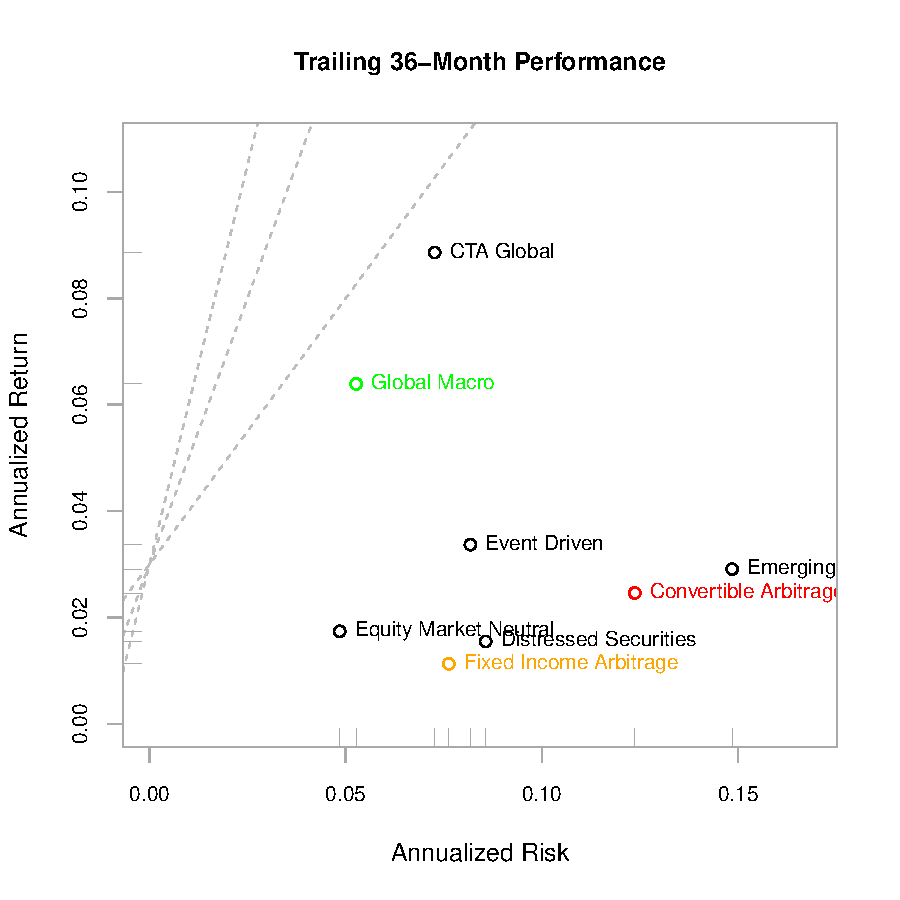
\includegraphics{UnSmoothReturnAnalysis-Graph3}

As we can see that, for a given amount of risk , all the funds deliver a positive return.The funds, standing out from the cluster, are the ones which have \textbf{lowest autocorrelation}, among the whole group.Also, given their stability, when we unsmooth the returns, it is expectedly seen, that they remain \textbf{unaffected}, by the change in model, while the rest of the funds, display a negative characteristic.

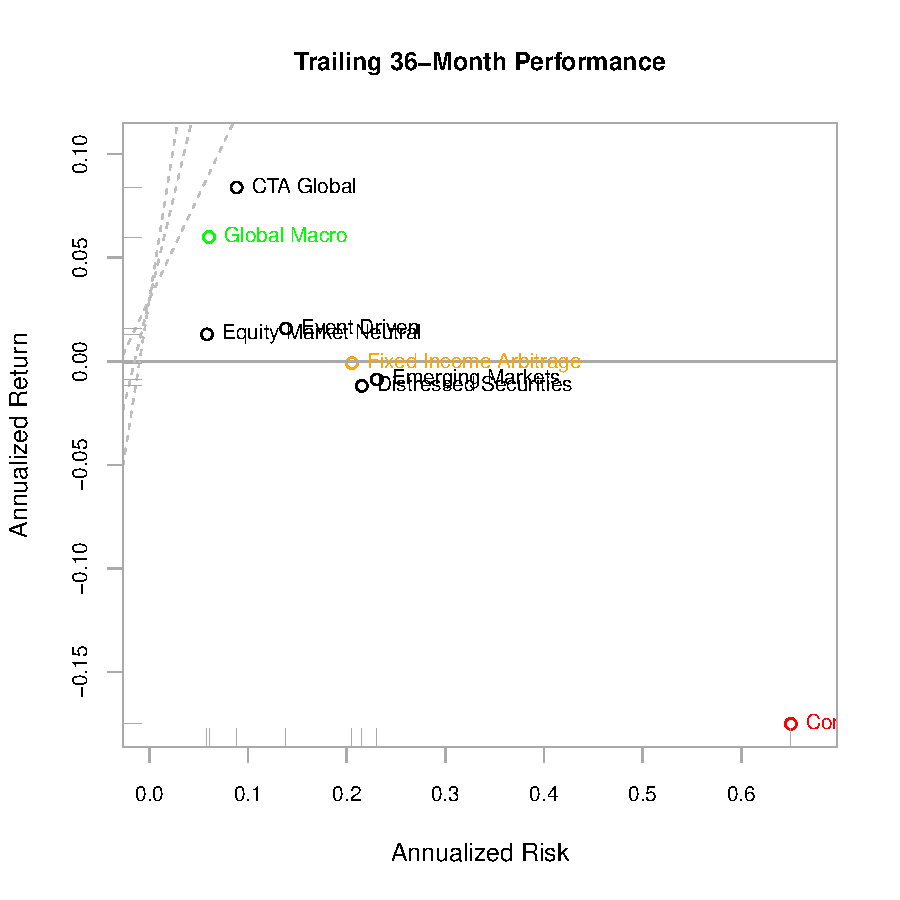
\includegraphics{UnSmoothReturnAnalysis-Graph4}

\subsection{Examine Performance Consistency}

Rolling performance is typically used as a way to assess stability of a return stream.Although perhaps it doesn't get much credence in the financial literature because of it's roots in digital signal processing, many practitioners and rolling performance to be a useful way to examine and segment performance and risk periods.

\begin{Schunk}
\begin{Sinput}
> charts.RollingPerformance(edhec[,1:4], Rf=.03/12, colorset = rich6equal, lwd = 2)
\end{Sinput}
\end{Schunk}
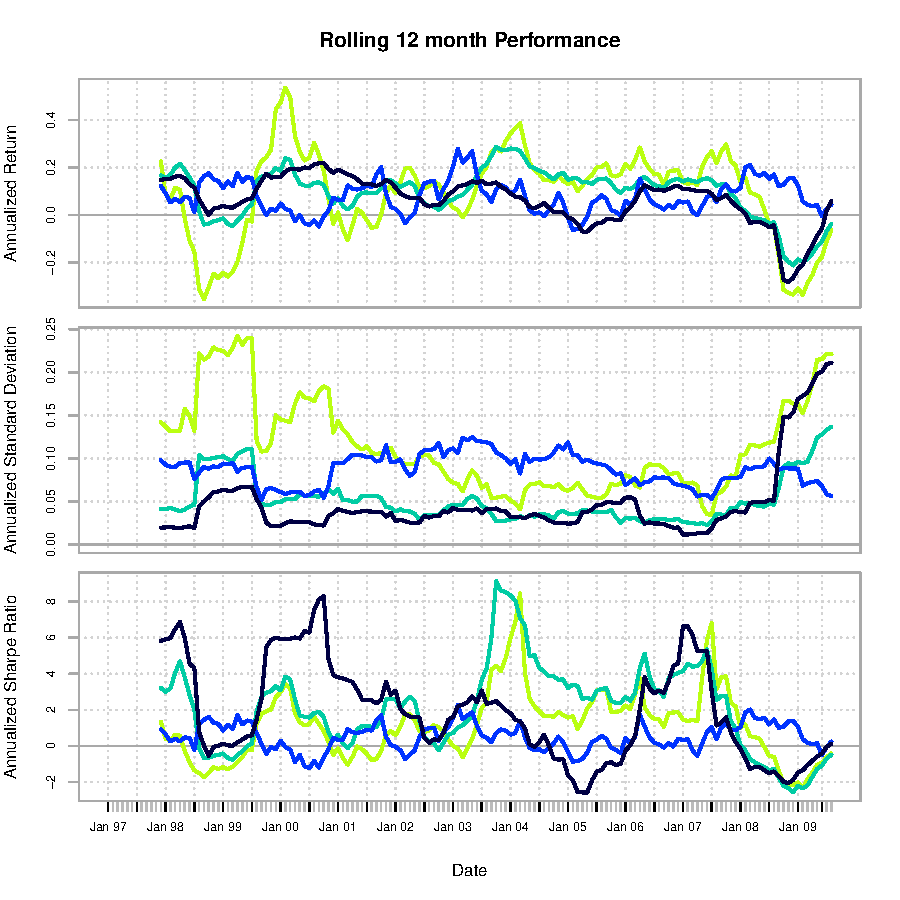
\includegraphics{UnSmoothReturnAnalysis-Graph5}


We can observe that \textbf{CTA Global} has once again, outperformed it's peer in the 3 charts respectively as well in the case of Okunev Return Model altough a steep fall is evident in the end time period for returns and subsequent rise in volatility.

\begin{Schunk}
\begin{Sinput}
> charts.RollingPerformance(Return.Okunev(edhec[,1:4]), Rf=.03/12, colorset = rich6equal, lwd = 2)
\end{Sinput}
\end{Schunk}
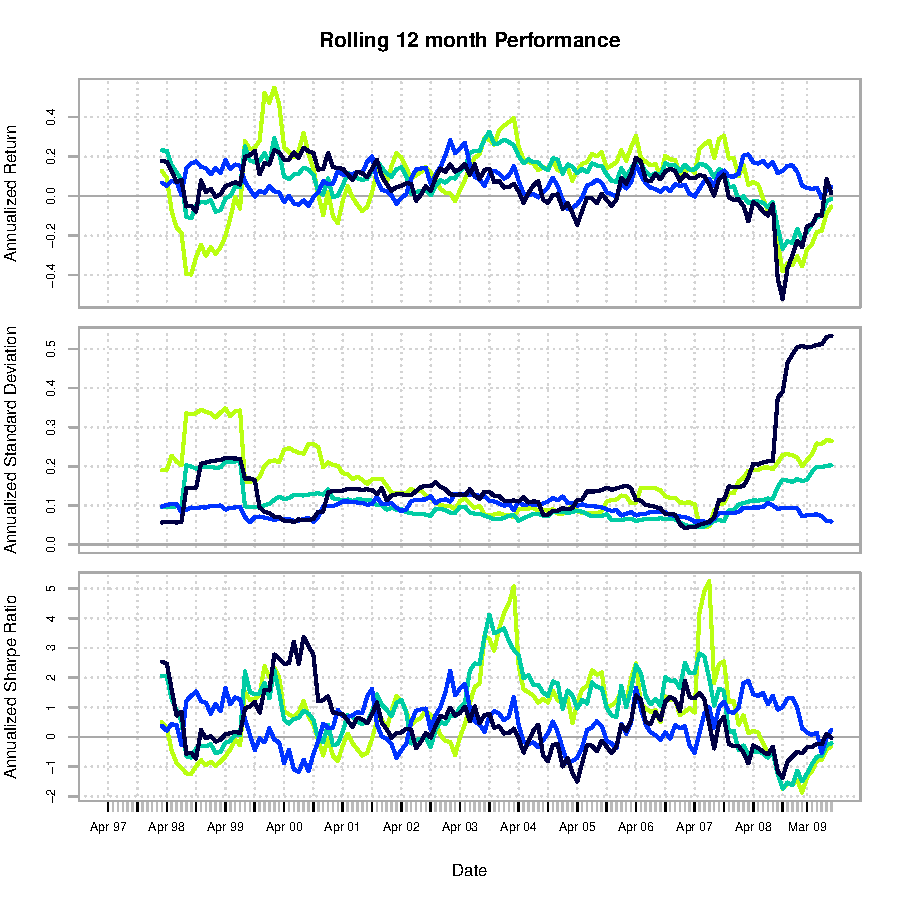
\includegraphics{UnSmoothReturnAnalysis-Graph6}

\end{document}
